%Tex root = BasiDiDati.tex

\chapter{Esecuzione concorrente di transazioni}
L'unità di misura usata per valutare il carico di lavoro din un DBMS è il \textcolor{azzurrino}{\textbf{transazioni al secondo}} (tps).\\[0.2ex]
PEr gestire con prestazioni accettabili il carico di lavoro tipico delle applicazioni gestionali è di 100 o 1000 tps.\\[0.2ex]
L'esecuzione concorrente di transazioni senza controllo può generare \textbf{naomalie} o \textbf{problemi di correttezza}.\\[0.2ex]
Bisogna, quindi, introdurre dei meccanismi di controllo nell'esecuzione delle transazioni per evitare tali anomalie.

\section{Tipologie di anomalie}
Le principali tipologie ddi anomalie sono:
\begin{itemize}[label=$\triangleright$, itemsep=\smallskipamount]
    \item \textbf{perdita di aggiornamento}: effetti di una transazione concorrente vengono persi (riscritti)
    \item \textbf{lettura inconsistente}: accessi sucessivi alla stessa risorsa ritornano risultati diversi
    \item \textbf{lettura sporca}: viene letto un dato che rappresenta uno stato intermedio di un'altra transazione
    \item \textbf{aggiornamento fantasma}: osservazione di uno stato intermedio che viola i vincoli d'integrità
    \item \textbf{inserimento fantasma}: valutazioni diverse di operazioni di aggregazione producono risultati diversi
\end{itemize}

\vario{Notazione}{
    \begin{itemize}[label=$\diamond$, itemsep=\smallskipamount]
        \item $\boldsymbol{\mathrm{t_i}}$: transazione $\mathrm{t_i}$
        \item $\boldsymbol{\mathrm{r_i(x)}}$: operazione di lettura eseguita dalla transazione $\mathrm{t_i}$ sulla risorsa $\mathrm{x}$
        \item $\boldsymbol{\mathrm{w_i(x)}}$: operazione di scrittura eseguita dalla transazione $\mathrm{t_i}$ sulla risorsa $\mathrm{x}$
    \end{itemize}
}

\subsection{Perdita di aggiornamento}
Nella \textbf{perdita di aggiornamento} gli effetti di una transazione concorrente vengono persi.

\esempio{perdita di aggiornamento}{
    Consieriamo le seguenti transazioni:
    \[
        \begin{aligned}
            \mathrm{t_1}: \quad \texttt{BOT}; \quad \mathrm{r_1(x)}; \quad \mathrm{x = x + 1}; \quad \mathrm{w_1(x)}; \quad \texttt{COMMIT}; \quad \texttt{EOT}\\
            \mathrm{t_2}: \quad \texttt{BOT}; \quad \mathrm{r_2(x)}; \quad \mathrm{x = x + 1}; \quad \mathrm{w_2(x)}; \quad \texttt{COMMIT}; \quad \texttt{EOT}
        \end{aligned}
    \]

    Simuliamo l'esecuzione concorrente di $\mathrm{t_1}$ e $\mathrm{t_2}$:
    \begin{figure}[H]
        \centering
        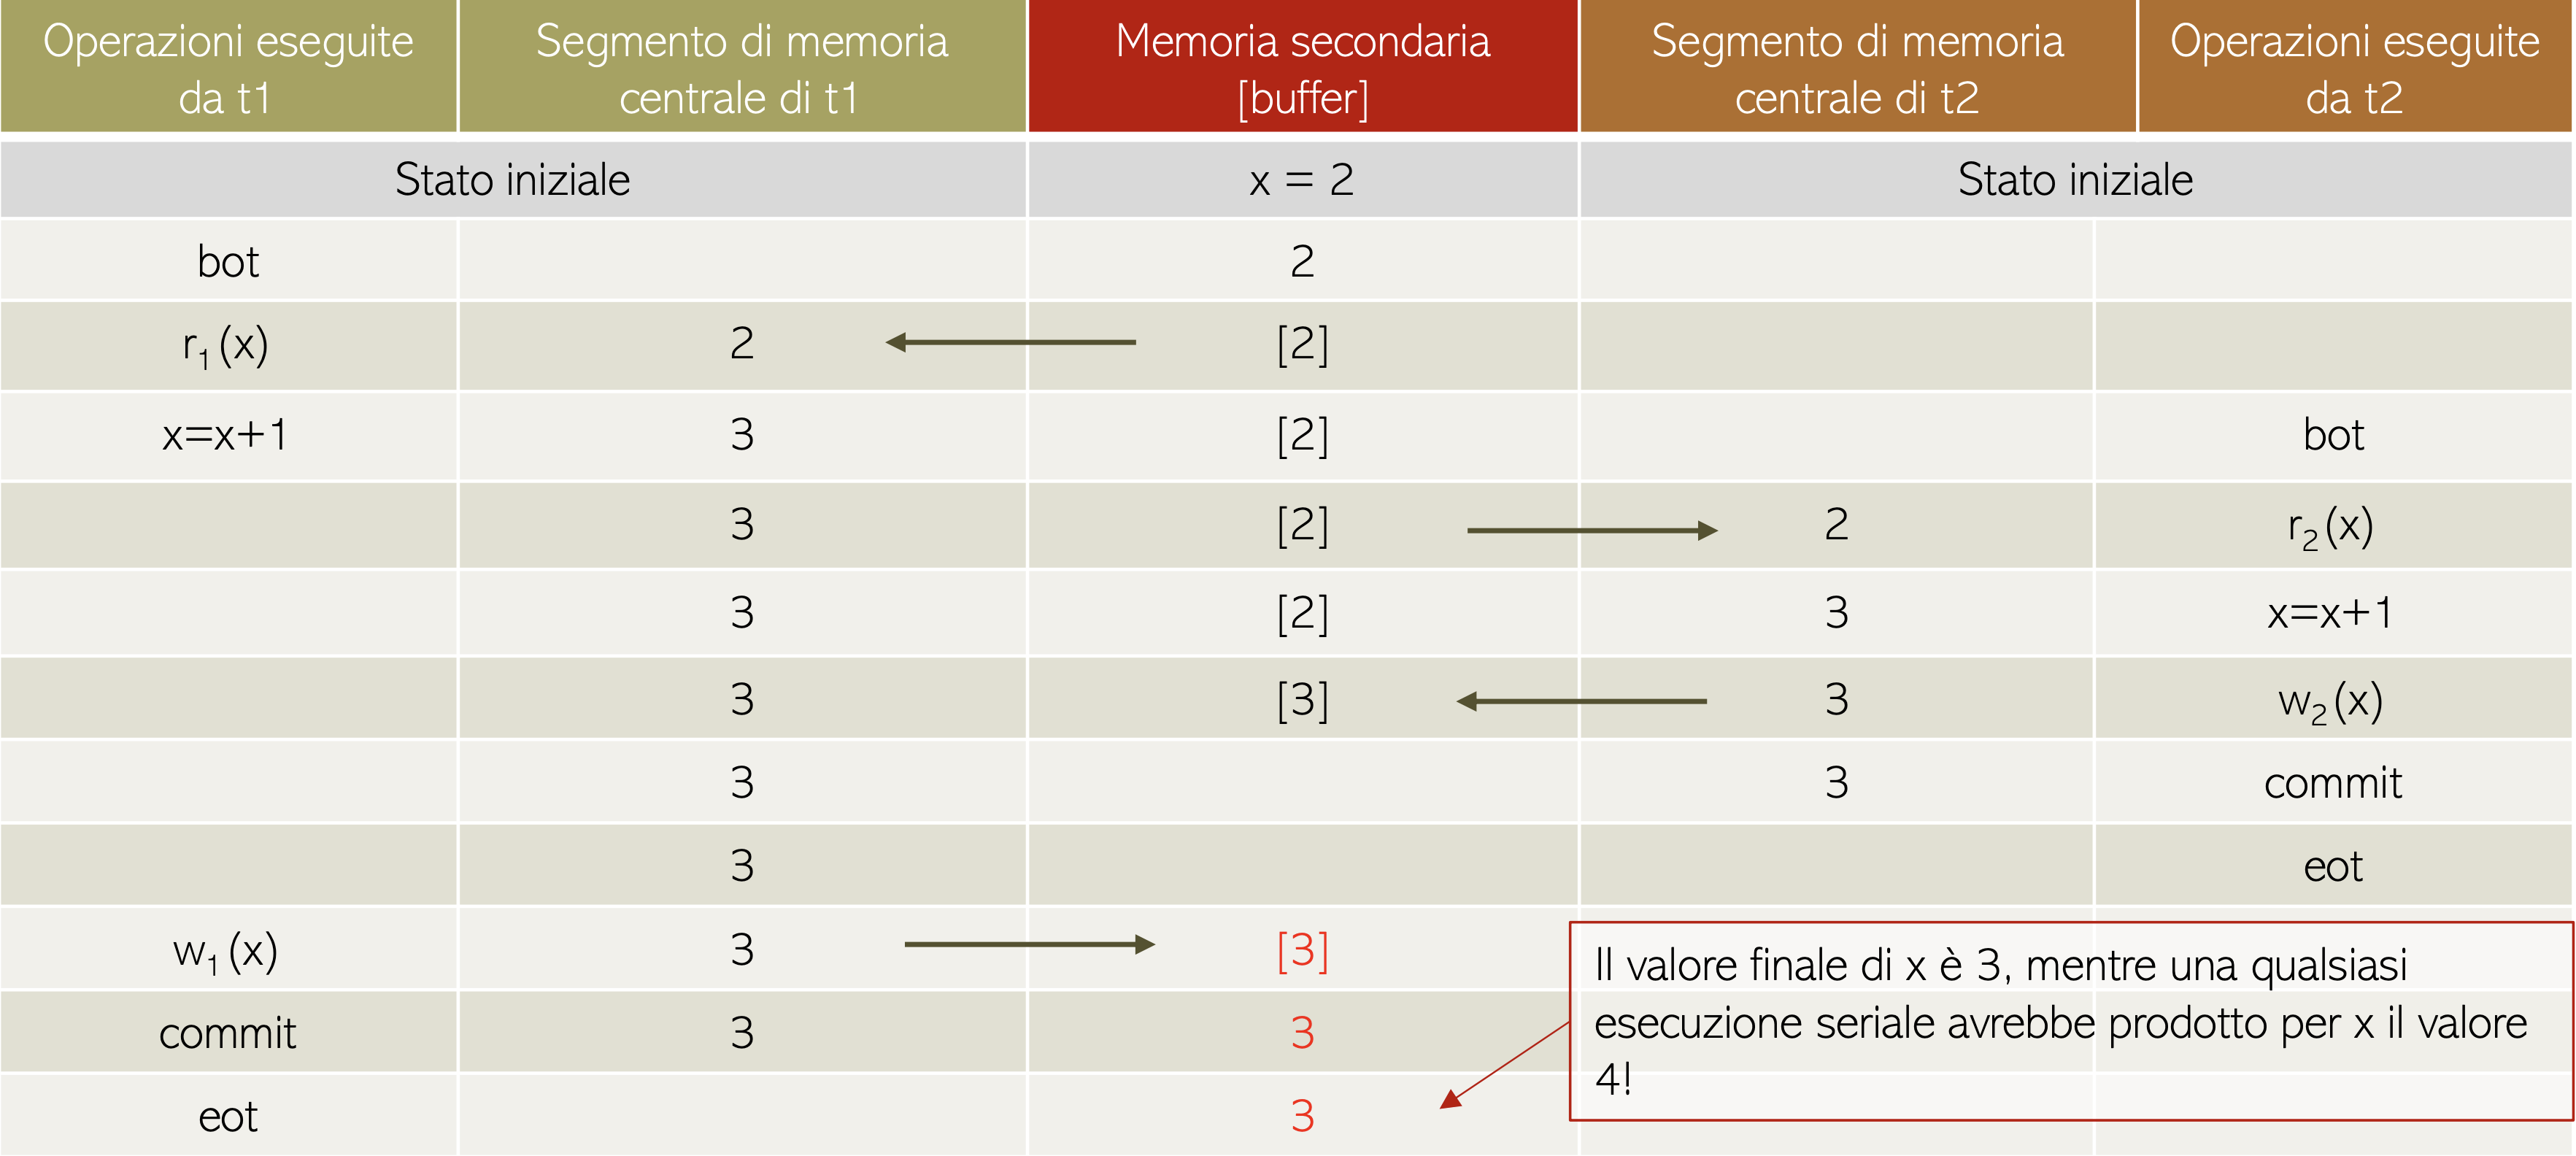
\includegraphics[width=0.9\textwidth]{images/perdita-aggiornamento.png}
    \end{figure}
}

\subsection{Lettura inconsistente}
Nella \textbf{lettura inconsistente} gli accessi sucessivi ad uno stesso dato all'interno di una transazione ritornano valori diversi.

\esempio{lettura inconsistente}{
    Consieriamo le seguenti transazioni:
    \[
        \begin{aligned}
            \mathrm{t_1}: \quad \texttt{BOT}; \quad \mathrm{r_1(x)}; \quad \mathrm{r_1'(x)}; \quad \mathrm{w_1(x)}; \quad \texttt{COMMIT}; \quad \texttt{EOT}\\
            \mathrm{t_2}: \quad \texttt{BOT}; \quad \mathrm{r_2(x)}; \quad \mathrm{x = x + 1}; \quad \mathrm{w_2(x)}; \quad \texttt{COMMIT}; \quad \texttt{EOT}
        \end{aligned}
    \]

    Simuliamo l'esecuzione concorrente di $\mathrm{t_1}$ e $\mathrm{t_2}$:
    \begin{figure}[H]
        \centering
        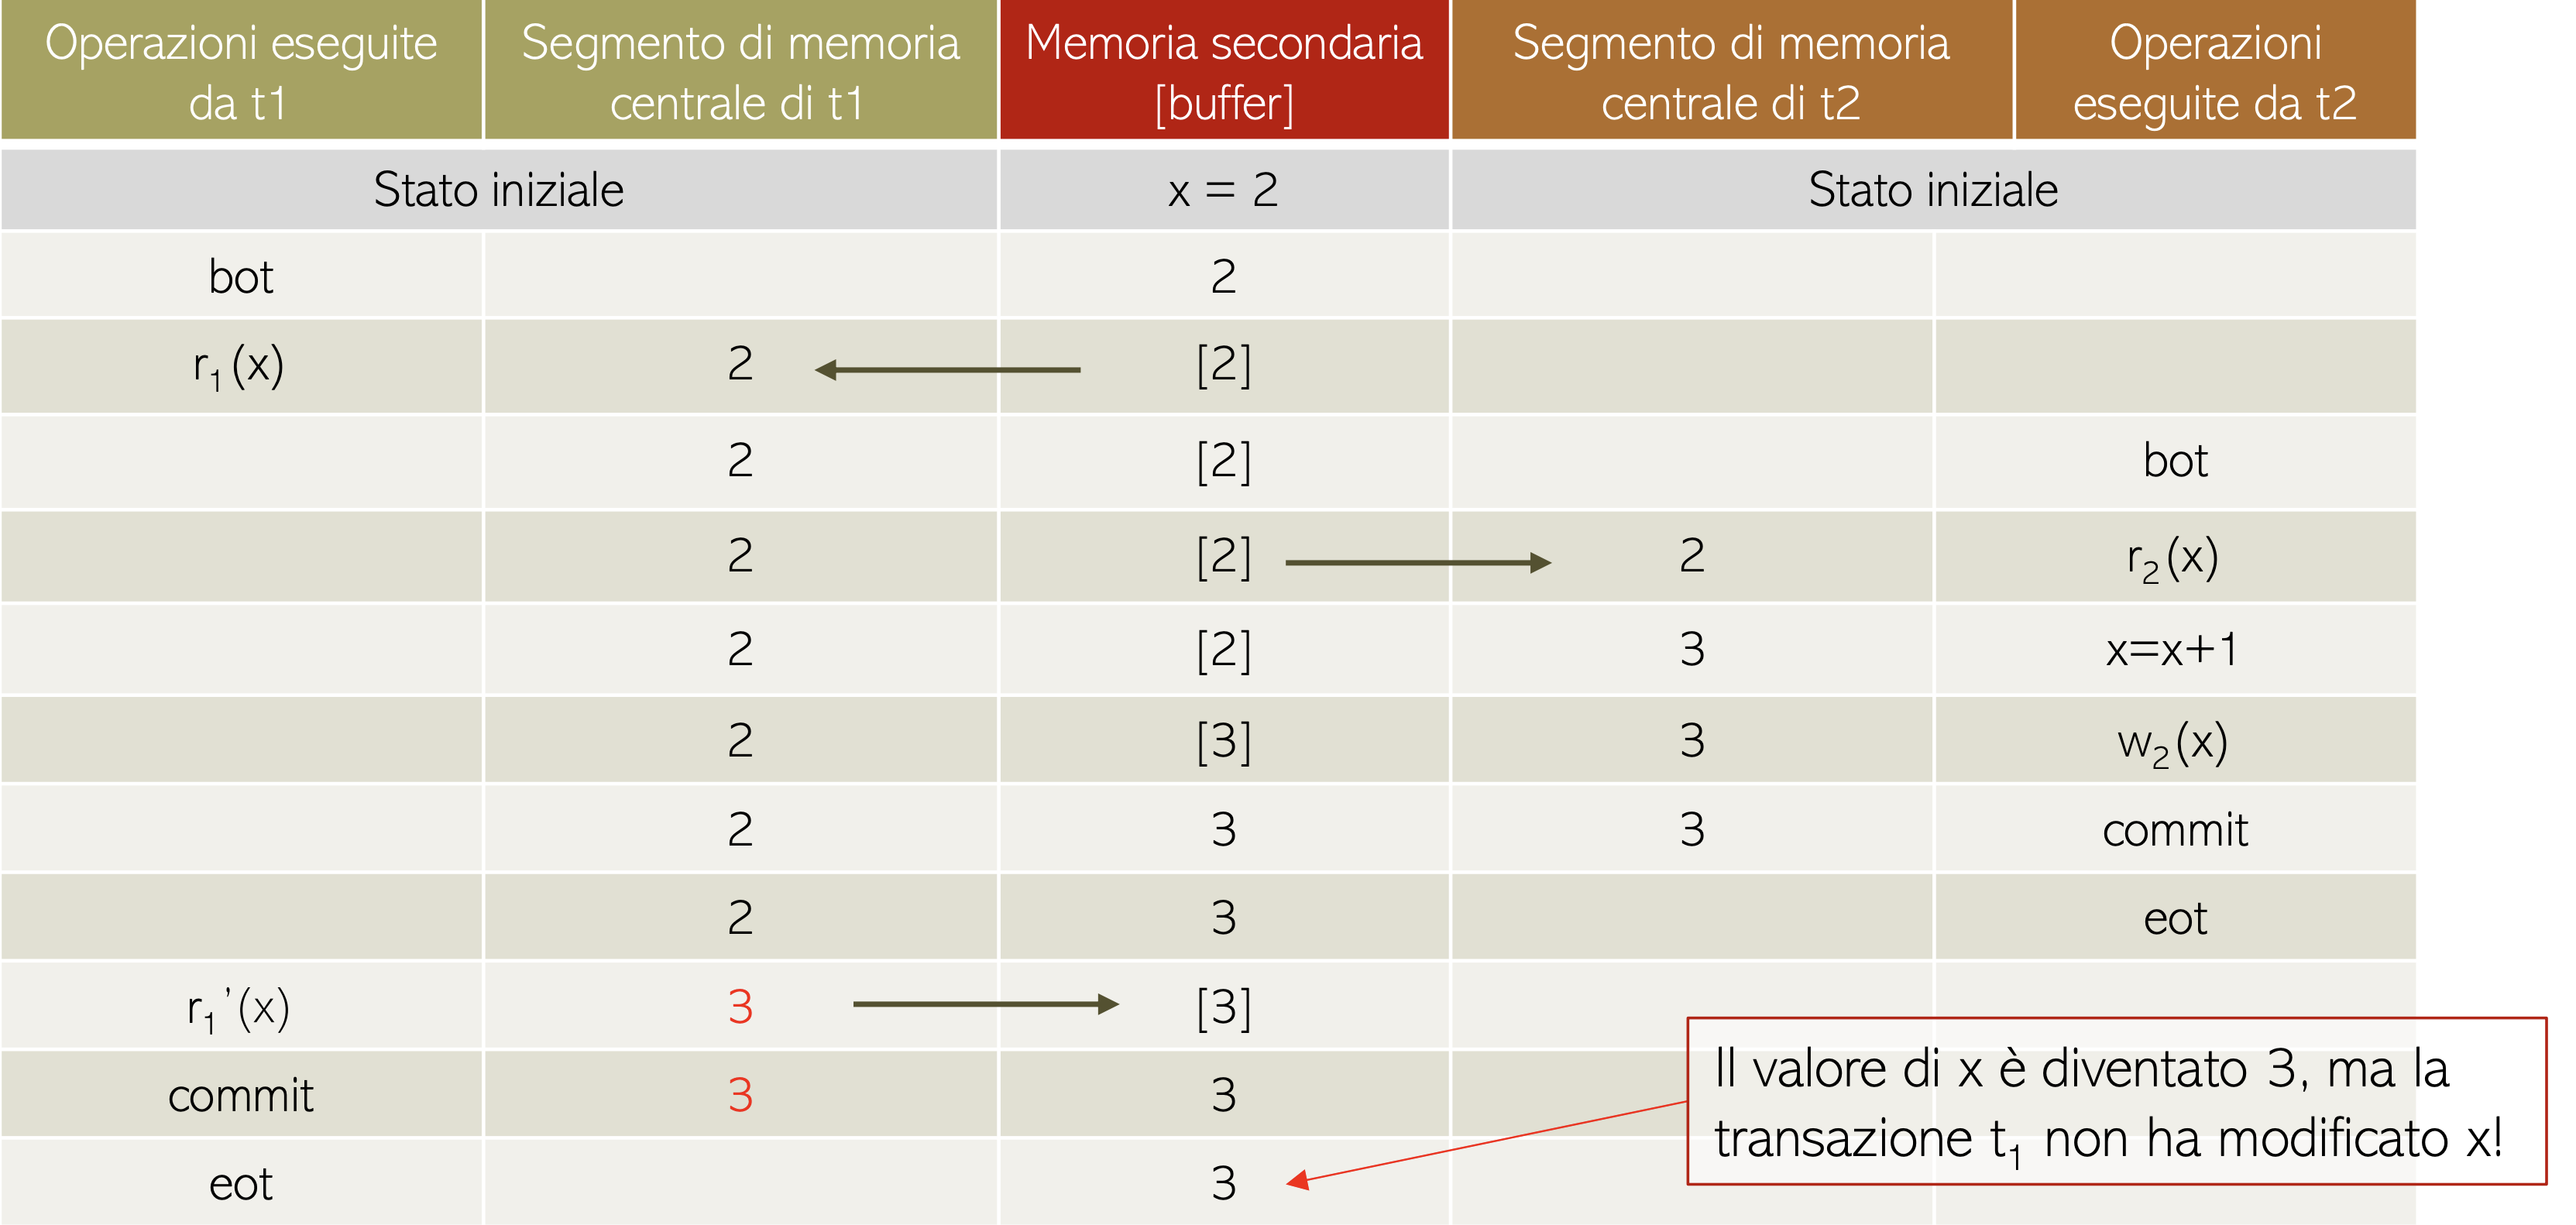
\includegraphics[width=0.9\textwidth]{images/lettura-inconsistente.png}
    \end{figure}
}

\subsection{Lettura sporca}
Nella \textbf{lettura sporca} viene letto un dato che rappresenta uno stato intermedio nell'evoluzione di una transazione.

\esempio{lettura inconsistente}{
    Consieriamo le seguenti transazioni:
    \[
        \begin{aligned}
            \mathrm{t_1}: \quad \texttt{BOT}; \quad \mathrm{r_1(x)}; \quad \texttt{COMMIT}; \quad \texttt{EOT}\\
            \mathrm{t_2}: \quad \texttt{BOT}; \quad \mathrm{r_2(x)}; \quad \mathrm{x = x + 1}; \quad \mathrm{w_2(x)}; \quad \dots \quad \texttt{ABORT}
        \end{aligned}
    \]

    Simuliamo l'esecuzione concorrente di $\mathrm{t_1}$ e $\mathrm{t_2}$:
    \begin{figure}[H]
        \centering
        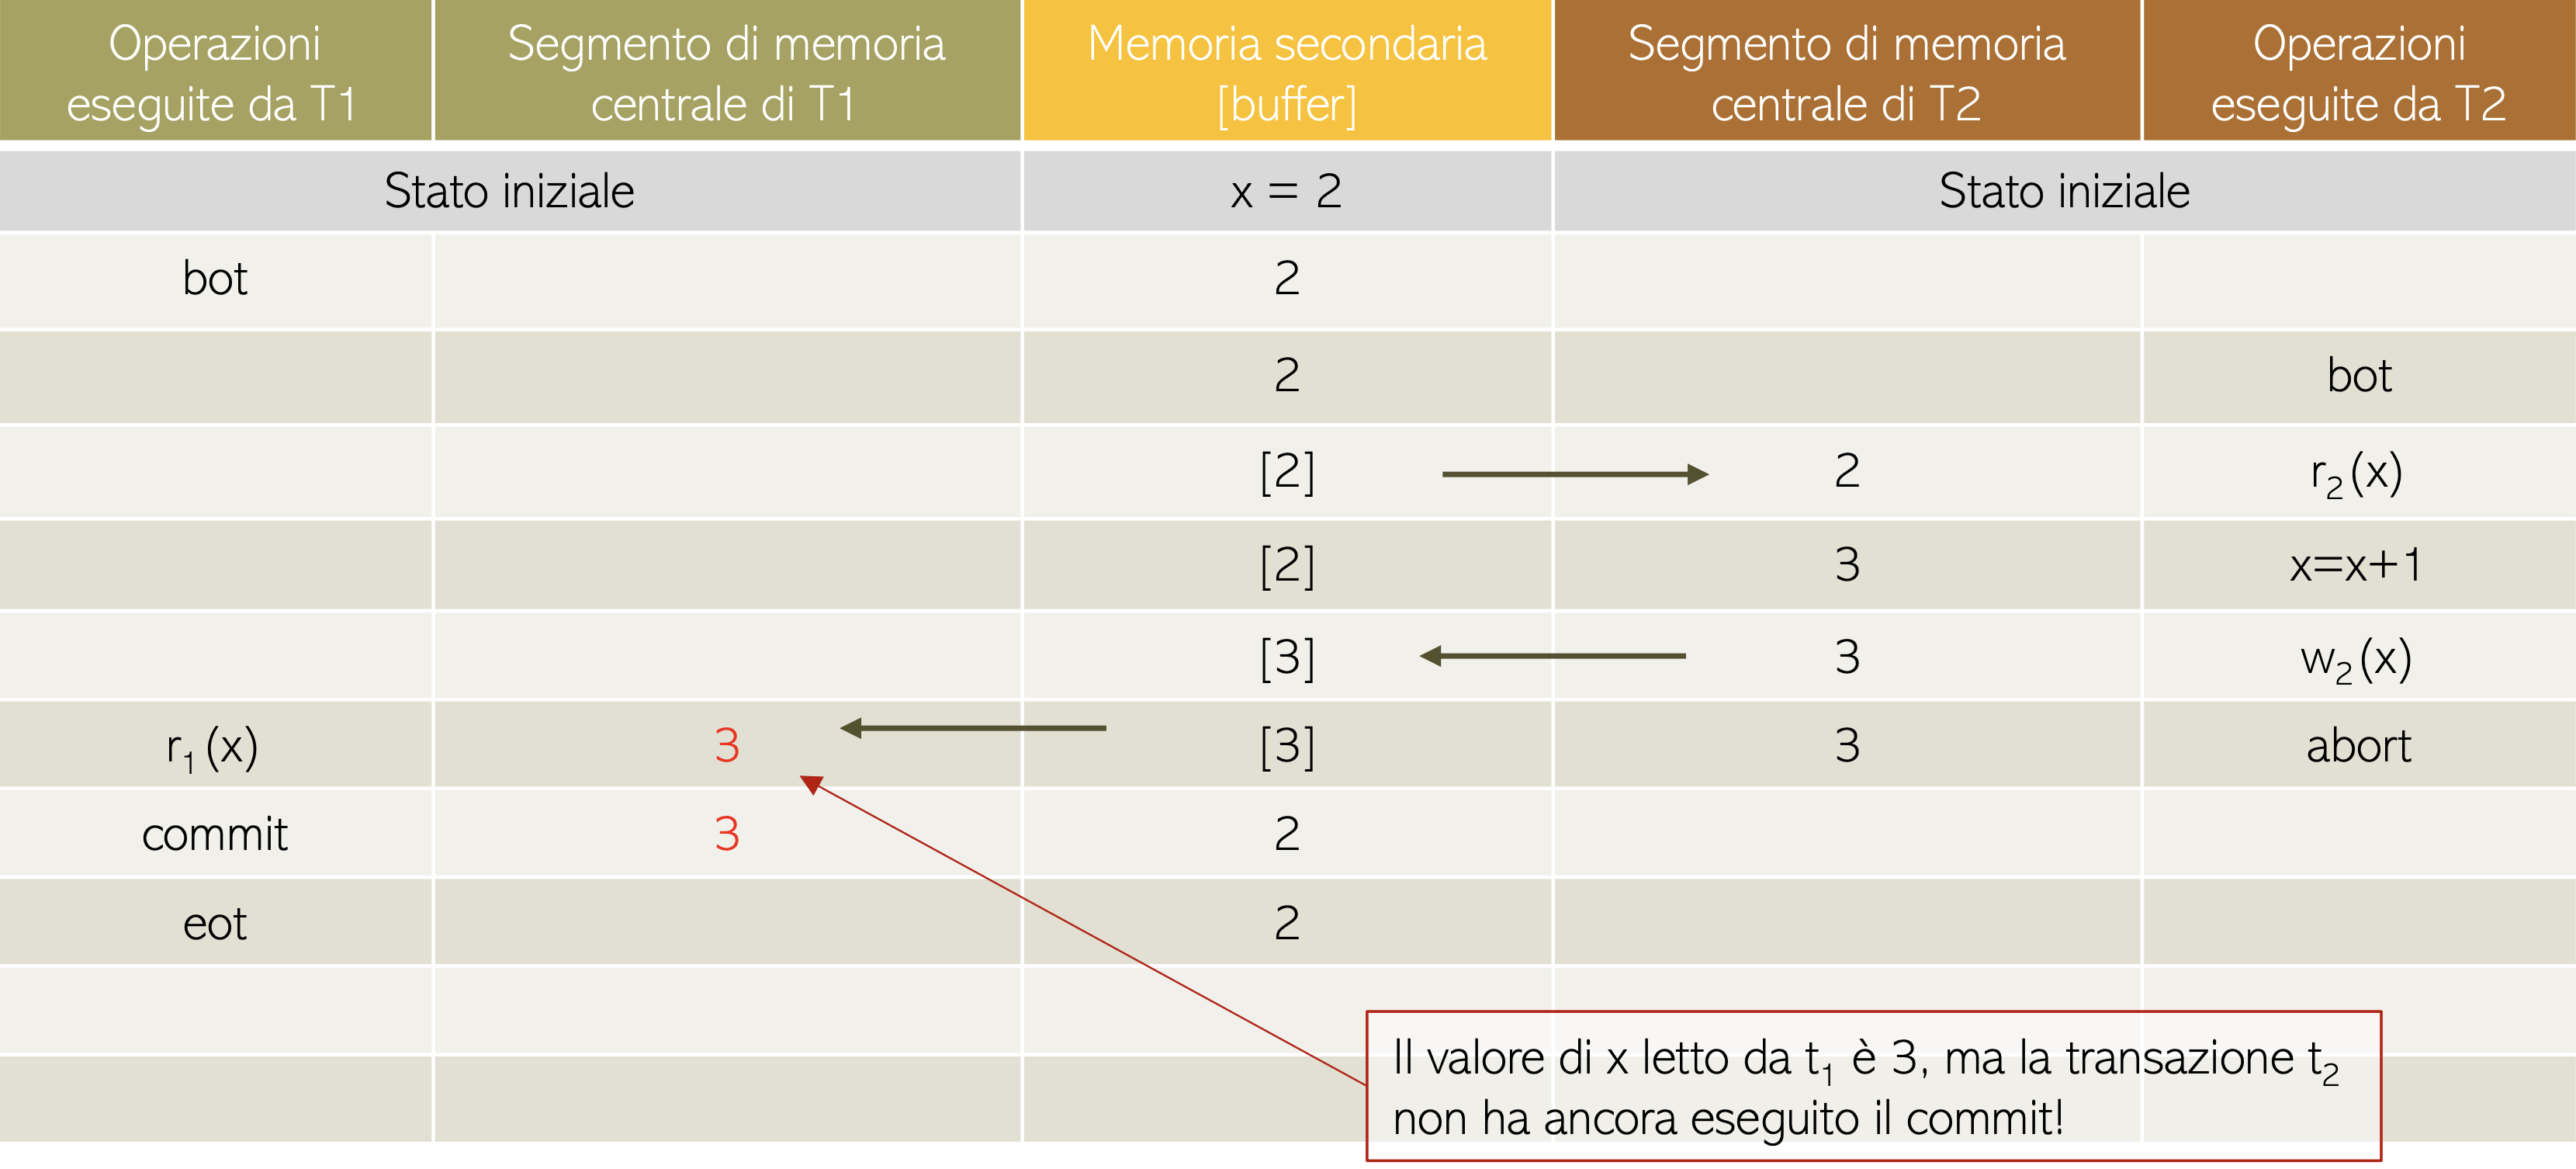
\includegraphics[width=0.9\textwidth]{images/lettura-sporca.png}
    \end{figure}
}

\subsection{Aggiornamento fantasma}
L'\textbf{aggiornamento fantasma} consiste nell'osservazione di uno stato intermedio che non soddifa i vincoli d'integrità.

\esempio{lettura inconsistente}{
    Consieriamo le seguenti transazioni:
    \[
        \begin{aligned}
            \text{risorse}: \mathrm{x}, \mathrm{y}, \mathrm{z}\\
            \text{vincoli}: \mathrm{x + y + z = 100}\\
            \mathrm{t_1}: \quad \texttt{BOT}; \quad \mathrm{r_1(y)}; \quad \mathrm{r_1(x)}; \quad \mathrm{r_1(s)}; \quad \mathrm{s = x + y +z}; \quad \texttt{EOT}\\
            \mathrm{t_2}: \quad \texttt{BOT}; \quad \mathrm{r_2(y)}; \quad \mathrm{y = y + 10}; \quad \mathrm{z = z - 10}; \quad \mathrm{w_2(x)}; \quad \mathrm{w_2(z)}; \quad \texttt{COMMIT} \quad \texttt{EOT}
        \end{aligned}
    \]

    Simuliamo l'esecuzione concorrente di $\mathrm{t_1}$ e $\mathrm{t_2}$:
    \begin{figure}[H]
        \centering
        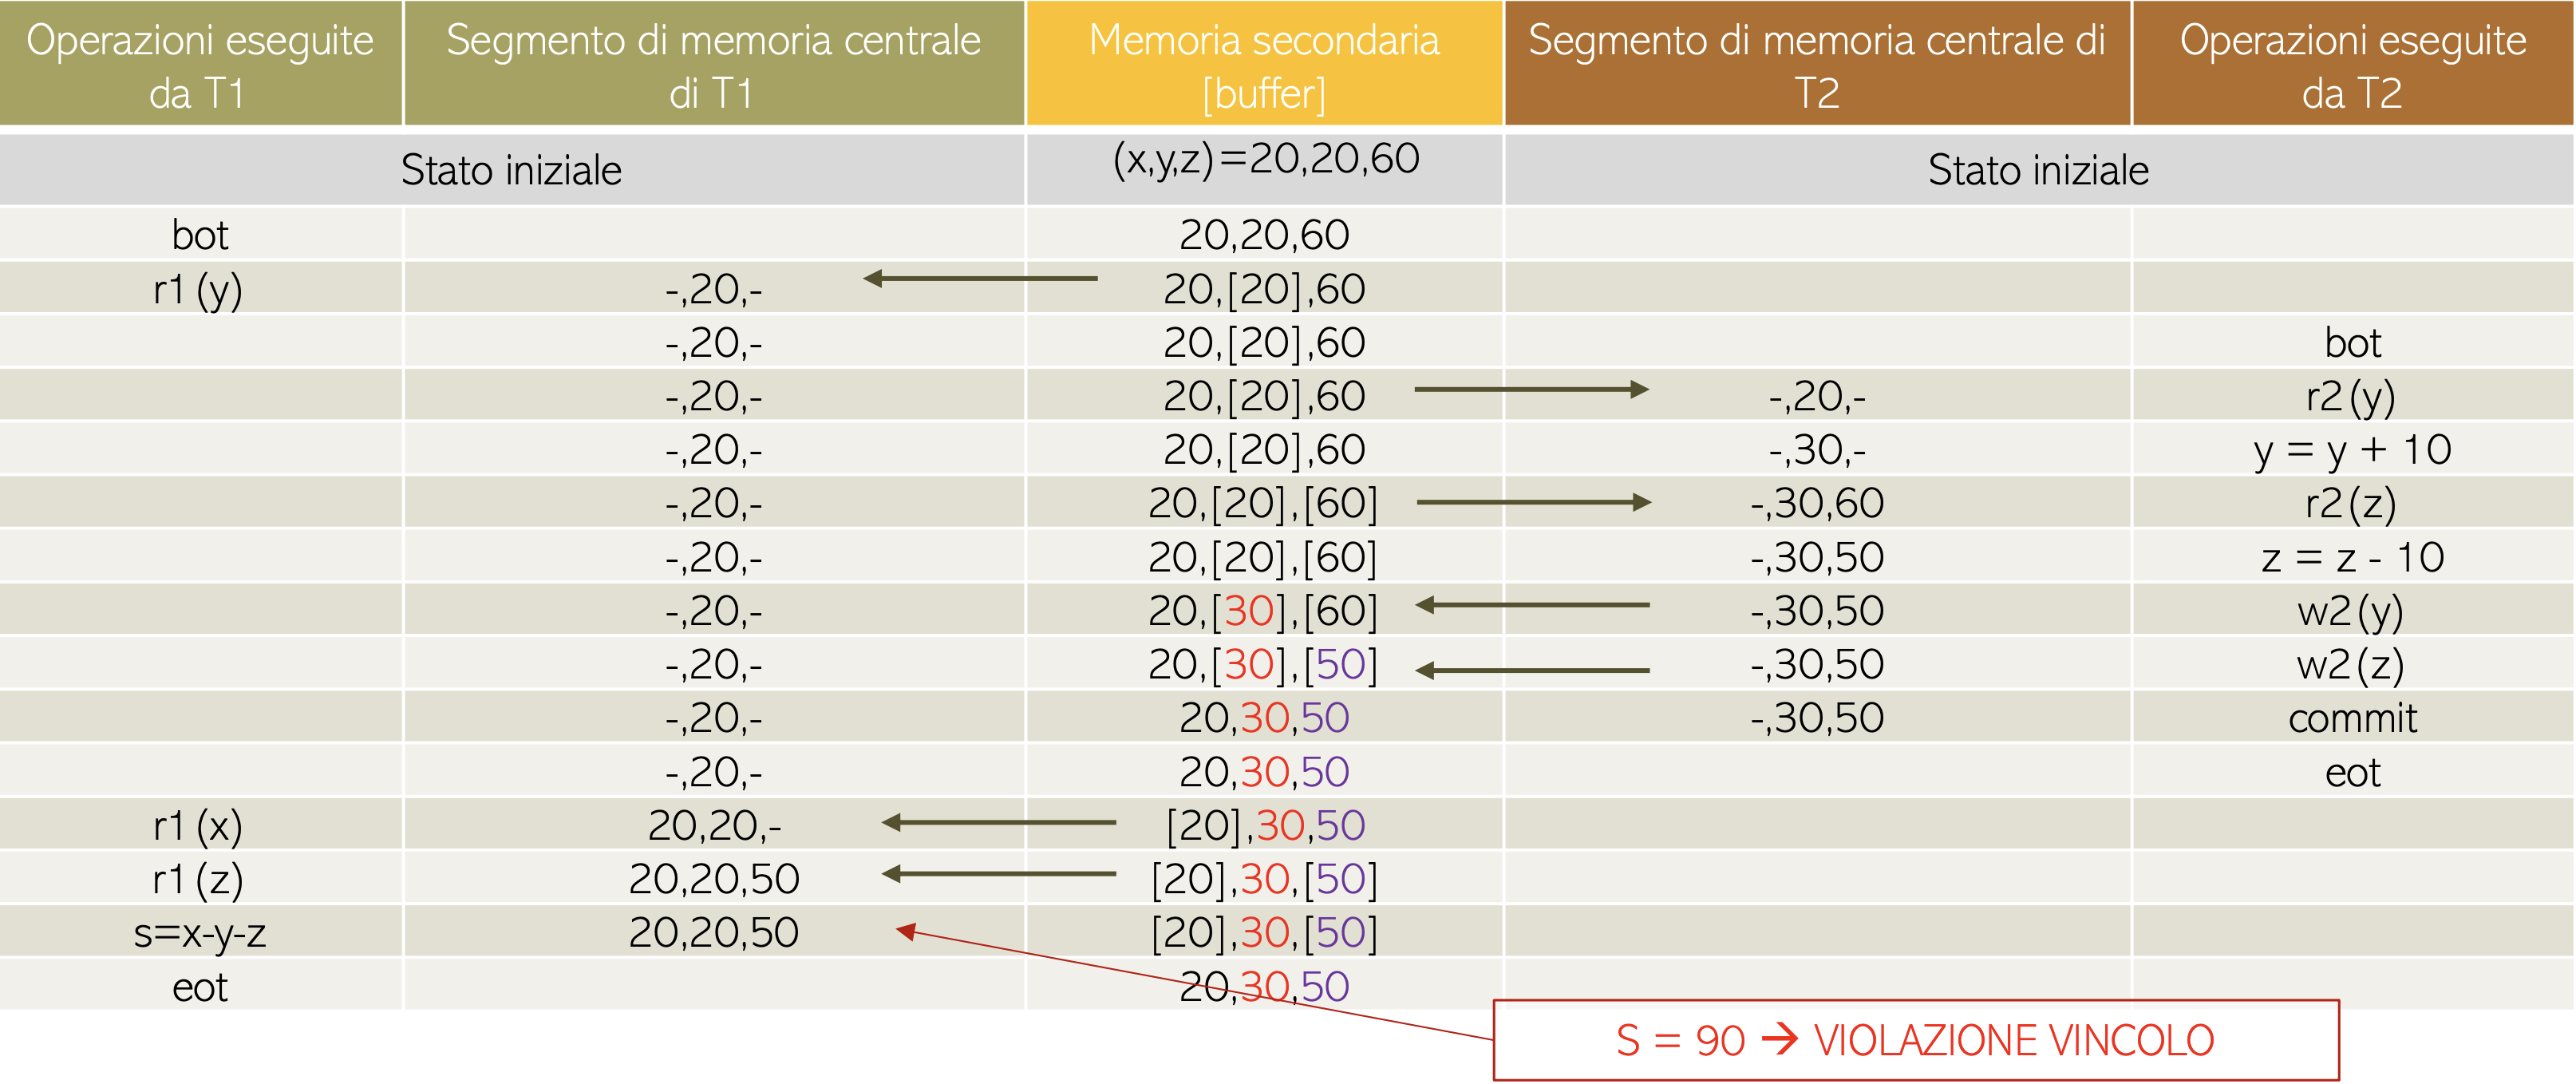
\includegraphics[width=0.9\textwidth]{images/aggiornamento-fantasma.png}
    \end{figure}
}

\subsection{Inserimento fantasma}
L'\textbf{inserimento fantasma} si verifica quando avvengono valutazioni diverse di valori aggregati a causa di inserimenti intermedi.\\[0.2ex]
La transazione che valuta un valore aggregato relativo a tutti gli elementi che soddifano un predicato di selezione (es. voto medio degli studenti) può subire l'anomalia di inserimento se il valore aggregato viene valutato due volte e tra la prima e la seconda valutazione viene inserito un nuovo studente.

\section{Schedule}
\definizione{schedule}{
    Lo \textbf{schedule} è una sequenza di operazioni di lettura e scrittura eseguite su risorse della base di dati da diverse transazioni concorrenti.
}

Lo schedule, quindi, rappresenta una possibile esecuzione concorrente di diverse transazioni:
\begin{equation*}
    \mathrm{S: r_1(x) \quad r_2(x) \quad w_1(z) \quad w_2(x)}
\end{equation*}

Per evitare anomalie, si stabilisce di accettare solo gli schedule equivalenti a uno schedule seriale.

\subsection{Schedule seriale}
\definizione{schedule seriale}{
    Uno \textbf{schedule seriale} è uno Schedule dove le operazioni di ogni transazione compaiono un seuqenza senza essere inframezzate da operazioni di altre transazioni.

    \noindent\rule{\textwidth}{0.4pt}

    \medskip
    \[
        \begin{aligned}
            \mathrm{s_1}: \mathrm{r_1(x)} \quad \mathrm{r_2(x)} \quad \mathrm{w_2(x)} \quad \mathrm{w_1(x)} &= \textbf{\text{NON è SERIALE}}\\
            \mathrm{s_2}: \mathrm{r_1(x)} \quad \mathrm{w_1(x)} \quad \mathrm{r_2(x)} \quad \mathrm{w_2(x)} &= \textbf{\text{è SERIALE}}
        \end{aligned}
    \]
}

\definizione{schedule serializzabile}{
    Lo \textbf{schedule serializzabile} è uno schedule equivalente a uno schedule seriale.
}

Due schedule si definiscono equivalenti se \textbf{producono gli stessi effetti} sulla base di dati.

\section{Tecniche di gestione della concorrenza}